\documentclass[conference]{IEEEtran}
\renewcommand{\ttdefault}{cmtt}

\usepackage[utf8]{inputenc}
\usepackage{amsmath,amssymb,amsfonts}
\usepackage{enumitem}
\usepackage{graphicx}
\usepackage{textcomp}
\usepackage{xcolor}
\usepackage[hidelinks]{hyperref}
\usepackage{booktabs}
\usepackage{multirow}
\usepackage{microtype}
\usepackage{tikz}
\usetikzlibrary{arrows.meta,positioning,fit}

\setlength{\abovedisplayskip}{4pt}
\setlength{\belowdisplayskip}{4pt}

% GENERATED by scripts/make_macros.py from eval/results/*.json -- do not edit
\newcommand{\hwName}{M4 Pro}
\newcommand{\nargoVer}{1.0.0-beta.22}
\newcommand{\bbVer}{5.0.0-nightly.20260522}
\newcommand{\benchRuns}{10}
\newcommand{\gatesSixtyFour}{155,575}
\newcommand{\proveSixtyFour}{0.58}
\newcommand{\verifySixtyFour}{10}
\newcommand{\witnessSixtyFour}{0.20}
\newcommand{\memSixtyFour}{335}
\newcommand{\proofKBSixtyFour}{14.3}
\newcommand{\gatesOneTwentyEight}{162,919}
\newcommand{\proveOneTwentyEight}{0.59}
\newcommand{\verifyOneTwentyEight}{10}
\newcommand{\witnessOneTwentyEight}{0.21}
\newcommand{\memOneTwentyEight}{344}
\newcommand{\proofKBOneTwentyEight}{14.3}
\newcommand{\gatesTwoFiftySix}{177,533}
\newcommand{\proveTwoFiftySix}{0.67}
\newcommand{\verifyTwoFiftySix}{10}
\newcommand{\witnessTwoFiftySix}{0.22}
\newcommand{\memTwoFiftySix}{366}
\newcommand{\proofKBTwoFiftySix}{14.3}
\newcommand{\gatesFiveTwelve}{206,835}
\newcommand{\proveFiveTwelve}{0.74}
\newcommand{\verifyFiveTwelve}{10}
\newcommand{\witnessFiveTwelve}{0.26}
\newcommand{\memFiveTwelve}{445}
\newcommand{\proofKBFiveTwelve}{14.3}
\newcommand{\gatesTenTwentyFour}{265,439}
\newcommand{\proveTenTwentyFour}{0.95}
\newcommand{\verifyTenTwentyFour}{10}
\newcommand{\witnessTenTwentyFour}{0.34}
\newcommand{\memTenTwentyFour}{648}
\newcommand{\proofKBTenTwentyFour}{14.3}
\newcommand{\gatesBdNone}{7,388}
\newcommand{\gatesBdSsn}{12,855}
\newcommand{\gatesBdEmail}{12,777}
\newcommand{\gatesBdPhoneus}{13,800}
\newcommand{\gatesBdIpvfour}{13,142}
\newcommand{\gatesBdDate}{13,212}
\newcommand{\gatesBdCard}{151,557}
\newcommand{\gatesBdAll}{177,533}
\newcommand{\gatesIncSsn}{5,467}
\newcommand{\gatesIncEmail}{5,389}
\newcommand{\gatesIncPhoneus}{6,412}
\newcommand{\gatesIncIpvfour}{5,754}
\newcommand{\gatesIncDate}{5,824}
\newcommand{\gatesIncCard}{144,169}
\newcommand{\refusalAi}{85.0\%}
\newcommand{\falseRefusalAi}{22.6\%}
\newcommand{\inScopeAi}{446}
\newcommand{\recAiCard}{0.216}
\newcommand{\recNAiCard}{8/37}
\newcommand{\recAiDate}{0.390}
\newcommand{\recNAiDate}{69/177}
\newcommand{\recAiEmail}{0.991}
\newcommand{\recNAiEmail}{212/214}
\newcommand{\recAiPhoneus}{0.333}
\newcommand{\recNAiPhoneus}{66/198}
\newcommand{\recAiSsn}{0.727}
\newcommand{\recNAiSsn}{93/128}
\newcommand{\refusalSyn}{100.0\%}
\newcommand{\falseRefusalSyn}{0.0\%}
\newcommand{\inScopeSyn}{500}
\newcommand{\recSynCard}{1.000}
\newcommand{\recNSynCard}{50/50}
\newcommand{\recSynDate}{0.671}
\newcommand{\recNSynDate}{151/225}
\newcommand{\recSynEmail}{0.821}
\newcommand{\recNSynEmail}{349/425}
\newcommand{\recSynIpvfour}{1.000}
\newcommand{\recNSynIpvfour}{125/125}
\newcommand{\recSynPhoneus}{0.843}
\newcommand{\recNSynPhoneus}{295/350}
\newcommand{\recSynSsn}{1.000}
\newcommand{\recNSynSsn}{325/325}
\newcommand{\agreeCases}{300}
\newcommand{\agreeOk}{300}
\newcommand{\llmModel}{llama3.2:3b}
\newcommand{\llmResponses}{180}
\newcommand{\llmWithPii}{12}
\newcommand{\llmRefused}{12}
\newcommand{\llmBenign}{60}
\newcommand{\llmBenignRefused}{0}
\newcommand{\llmMedianBytes}{201}
\newcommand{\llmMaxBytes}{858}
\newcommand{\llmCaughtCard}{6/6}
\newcommand{\llmCaughtDate}{7/10}
\newcommand{\llmCaughtEmail}{4/7}
\newcommand{\llmCaughtIpvfour}{12/12}
\newcommand{\llmCaughtPhoneus}{6/7}
\newcommand{\llmCaughtSsn}{4/4}
\newcommand{\presRefusalAi}{97.5\%}
\newcommand{\presFalseRefusalAi}{34.8\%}
\newcommand{\presAiLocation}{0.210}
\newcommand{\presNAiLocation}{81/386}
\newcommand{\presAiPerson}{0.385}
\newcommand{\presNAiPerson}{271/704}
\newcommand{\presAiCard}{0.108}
\newcommand{\presNAiCard}{4/37}
\newcommand{\presAiDate}{0.825}
\newcommand{\presNAiDate}{146/177}
\newcommand{\presAiEmail}{0.935}
\newcommand{\presNAiEmail}{200/214}
\newcommand{\presAiPhoneus}{0.399}
\newcommand{\presNAiPhoneus}{79/198}
\newcommand{\presAiSsn}{0.703}
\newcommand{\presNAiSsn}{90/128}
\newcommand{\presRefusalSyn}{99.6\%}
\newcommand{\presFalseRefusalSyn}{23.0\%}
\newcommand{\presSynPerson}{0.897}
\newcommand{\presNSynPerson}{426/475}
\newcommand{\presSynCard}{0.720}
\newcommand{\presNSynCard}{36/50}
\newcommand{\presSynDate}{1.000}
\newcommand{\presNSynDate}{225/225}
\newcommand{\presSynEmail}{0.821}
\newcommand{\presNSynEmail}{349/425}
\newcommand{\presSynIpvfour}{1.000}
\newcommand{\presNSynIpvfour}{125/125}
\newcommand{\presSynPhoneus}{0.860}
\newcommand{\presNSynPhoneus}{301/350}
\newcommand{\presSynSsn}{1.000}
\newcommand{\presNSynSsn}{325/325}
\newcommand{\teeGates}{216,041}
\newcommand{\teeProve}{0.77}
\newcommand{\teeVerify}{11}
\newcommand{\teeMem}{432}
\newcommand{\teeNerMs}{7}
\newcommand{\teeSignMs}{0.9}
\newcommand{\teeExtraGates}{38,508}
\newcommand{\teeAttacks}{4}
\newcommand{\teeAttacksRefused}{4}

\newcommand{\sys}{\textsc{ZKPriv}}

\begin{document}

\title{ZKPriv: Zero-Knowledge Proofs That LLM Responses Contain No Prohibited Personal Data}

\author{%
  \IEEEauthorblockN{Huzaif Khan\IEEEauthorrefmark{1},\;
    Ghazal Mahdian\IEEEauthorrefmark{2},\;
    Ali Jalooli\IEEEauthorrefmark{3}}
  \IEEEauthorblockA{Department of Computer Science,
    California State University, Dominguez Hills,
    Carson, CA 90747, USA\\
    \IEEEauthorrefmark{1}hkhan17@toromail.csudh.edu,\;
    \IEEEauthorrefmark{2}gmahdian1@toromail.csudh.edu,\;
    \IEEEauthorrefmark{3}ajalooli@csudh.edu}
}

\maketitle

\begin{abstract}
Cloud-hosted large language models (LLMs) can reproduce personally identifiable information (PII) from their context or training data, and a provider can serve such a response to one user while appearing compliant to auditors. Zero-knowledge (ZK) systems for LLMs prove that a model computed an output correctly, but not what the output contains. We present \sys{}, a system in which every response carries a ZK proof that the committed response bytes contain no structured PII forbidden by the provider's registered policy, without revealing the prompt, the response, or the model. Unlike designs in which the provider supplies PII labels as a private input, \sys{} computes detection inside the circuit: each detector is compiled to a minimized search automaton, and the proof shows that no automaton reaches an accepting state anywhere in the response. A left-to-right automaton tracks the Luhn checksum so that payment cards are recognized without look-ahead. The circuit also binds the response length and padding, an optional ASCII guard, a Poseidon2 commitment, and a versioned policy hash. Implemented in Noir with zero-knowledge UltraHonk on an Apple \hwName{} CPU, a 256-byte response checked by six detectors compiles to \gatesTwoFiftySix{} gates, proves in \proveTwoFiftySix{}\,s, and verifies in \verifyTwoFiftySix{}\,ms with a \proofKBTwoFiftySix{}\,KiB proof. Names and places, which no pattern captures, are handled by a second tier: an enclave runs named-entity recognition and signs the labels over the response commitment, and the circuit verifies the signature and enforces the policy on them, adding \teeExtraGates{} gates and proving in \teeProve{}\,s. The circuit agrees with independent reference detectors on all \agreeCases{} test inputs, rejects all \teeAttacks{} label-forgery attacks we tried, and, compared with Presidio on the same 1{,}000 records, detects more payment cards while refusing far fewer texts whose labelled PII has been removed (\falseRefusalSyn{} vs.\ \presFalseRefusalSyn{} on synthetic data).
\end{abstract}

\begin{IEEEkeywords}
Large language models, zero-knowledge proofs, privacy compliance, PII detection, finite automata, verifiable computation
\end{IEEEkeywords}

% ════════════════════════════════════════════════════
\section{Introduction}
% ════════════════════════════════════════════════════

Cloud LLMs are increasingly used in healthcare, finance and customer service, where responses may only be released if they do not disclose regulated personal data. LLMs reproduce PII from their prompts, retrieved documents and training data~\cite{carlini2021extracting}. A provider can filter outputs, but a filter offers no evidence to anyone outside the provider: a provider that disables it for one user, or for one request, looks the same to an auditor as one that never did.

Privacy-enhancing technologies for LLM inference---MPC, FHE, trusted execution environments (TEEs) and prompt obfuscation~\cite{andreoletti2026privacysurvey}---hide the prompt or the response from the provider. They do not certify what the response contains. Zero-knowledge systems for LLMs, such as zkLLM~\cite{sun2024zkllm} and zkGPT~\cite{qu2025zkgpt}, prove that a committed output was computed by a committed model; they say nothing about whether that output contains a Social Security number. Output guardrails~\cite{nemogauardrails,llamaguard2} check content but are not verifiable.

The previous version of this work proved compliance with respect to sensitivity labels that the provider computed outside the proof and supplied as a private witness. A dishonest prover can set every label to ``not sensitive'', so such a proof certifies only what the provider claims. This paper removes that gap for structured PII, whose labels are \emph{computed inside the circuit} from the committed response bytes, and narrows it for names and places, whose labels must be signed by an attested enclave over the same commitment.

\textbf{Contributions.}
\begin{enumerate}[leftmargin=1.2em,itemsep=1pt]
  \item \textbf{In-circuit absence proofs for structured PII.} Detectors for SSNs, e-mail addresses, US phone numbers, IPv4 addresses, numeric dates and payment cards are compiled to minimized search automata with absorbing accept states, so ``the response contains no match'' reduces to a single check on the final state. A dedicated automaton tracks two Luhn sums left to right, recognizing valid card numbers without look-ahead.
  \item \textbf{A policy-bound response receipt.} The proof binds a Poseidon2~\cite{poseidon2} commitment to the response, its exact length and zero padding, the request identifier, and the hash of a versioned policy that selects detectors. The user who receives a response checks it against the commitment, so a provider cannot certify one response and deliver another.
  \item \textbf{A second tier for semantic PII.} Names and places are labelled by named-entity recognition inside an enclave, which signs the labels over the response commitment; the circuit verifies the secp256k1 signature and enforces the policy on the signed labels. The structured-PII guarantee holds without trusting the enclave; only the semantic tier depends on it.
  \item \textbf{An implementation and measurement.} We implement \sys{} in Noir~\cite{noir} with zero-knowledge UltraHonk~\cite{barretenberg} and report measured circuit size, proving and verification time, memory and proof size on commodity hardware, circuit-to-reference agreement, resistance to label forgery, and detection on two PII corpora, compared with Presidio, and on real LLM outputs. All code, data and scripts that produce the numbers in this paper are released.
\end{enumerate}

% ════════════════════════════════════════════════════
\section{Related Work}
% ════════════════════════════════════════════════════

\textbf{Private and verifiable LLM inference.} MPC~\cite{dong2023puma,gupta2023sigma}, FHE~\cite{decastro2025encryptedllm,park2025powerformer} and TEE-based inference~\cite{chrapek2025confidentialllm} protect prompts and responses from the provider; prompt-side techniques~\cite{tong2025inferdpt,zeng2025privacyrestore} reduce what is sent. zkLLM~\cite{sun2024zkllm} and zkGPT~\cite{qu2025zkgpt} prove inference correctness, and FairProof~\cite{yadav2024fairproof} certifies model fairness. None proves a property of an individual response's content. \sys{} is complementary: its commitment can be the output commitment of a correctness proof.

\textbf{ZK proofs over text.} Reef~\cite{reef} proves that a committed document matches, or does not match, a regular expression, and zk-regex~\cite{zkregex} and Londhe~\emph{et al.}~\cite{londhe2026regex} prove regex matches for e-mail verification. Path-witness constructions prove that a match \emph{exists}; they cannot prove absence. \sys{} applies a forced, whole-string automaton run, as in Reef's non-match case, to LLM responses, and adds what output compliance needs: detectors with checksum validation, length and padding binding, policy selection with versioning, and per-request binding. Zero-Knowledge Middleboxes~\cite{zkmiddlebox} prove that encrypted traffic complies with a policy; \sys{} transfers that model to LLM responses.

\textbf{Governance and filtering.} Blockchain audit logs~\cite{jan2025blockchainagentic,ameen2025audittrails} record that a check occurred but not that a specific response passed it. Guardrails~\cite{nemogauardrails,llamaguard2,selfcheckgpt} and PII detectors such as Presidio~\cite{presidio} and our earlier edge framework SenseCLLM~\cite{sensecllm} filter text but produce no verifiable evidence.

% ════════════════════════════════════════════════════
\section{System Model}
\label{sec:sysmodel}
% ════════════════════════════════════════════════════

\begin{figure}[t]
\centering
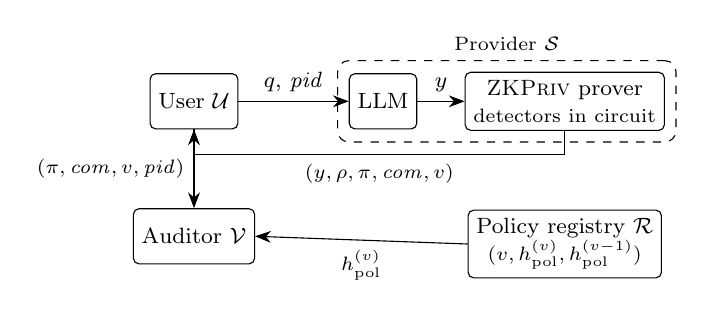
\begin{tikzpicture}[font=\footnotesize, node distance=4mm and 6mm,
  box/.style={draw, rounded corners=2pt, align=center, inner sep=3pt, minimum height=7mm},
  arr/.style={-{Stealth[length=2mm]}}]
\node[box] (u) {User $\mathcal{U}$};
\node[box, right=14mm of u] (llm) {LLM};
\node[box, right=of llm] (pr) {\sys{} prover\\{\scriptsize detectors in circuit}};
\node[draw, dashed, rounded corners, fit=(llm)(pr), inner sep=4pt, label={[font=\scriptsize]above:Provider $\mathcal{S}$}] (s) {};
\node[box, below=10mm of pr] (reg) {Policy registry $\mathcal{R}$\\{\scriptsize $(v, h_{\mathrm{pol}}^{(v)}, h_{\mathrm{pol}}^{(v-1)})$}};
\node[box, below=10mm of u] (aud) {Auditor $\mathcal{V}$};
\draw[arr] (u) -- node[above]{$q$, $\mathit{pid}$} (llm);
\draw[arr] (llm) -- node[above]{$y$} (pr);
\draw[arr] (pr.south) |- ++(0,-3mm) -| node[pos=0.25, below, font=\scriptsize]{$(y,\rho,\pi,\mathit{com},v)$} (u.south);
\draw[arr] (reg.west) -- node[below, font=\scriptsize]{$h_{\mathrm{pol}}^{(v)}$} (aud.east);
\draw[arr] (u) -- node[left, font=\scriptsize]{$(\pi,\mathit{com},v,\mathit{pid})$} (aud);
\end{tikzpicture}
\caption{\sys{} workflow. The provider proves that the committed response contains no structured PII forbidden by policy version $v$. The user checks the commitment opening and the proof; any auditor can verify a forwarded receipt without seeing the response.}
\label{fig:system}
\end{figure}

\textbf{Principals.} A user $\mathcal{U}$ sends prompt $q$ with a fresh request identifier $\mathit{pid}$ to a provider $\mathcal{S}$ that runs an LLM. $\mathcal{S}$ publishes policies in an append-only, hash-chained registry $\mathcal{R}$ of records $(v, h_{\mathrm{pol}}^{(v)}, h_{\mathrm{pol}}^{(v-1)}, \tau_v)$. An auditor $\mathcal{V}$ (a regulator or the user) holds the public verification key and reads $\mathcal{R}$ (Fig.~\ref{fig:system}).

\textbf{Protocol.} For response $y$ (UTF-8 bytes, $|y| \le N$), $\mathcal{S}$ samples a blinding value $\rho$ and computes
\begin{equation}
\begin{aligned}
  \mathit{com} &= H\bigl(\mathrm{pack}(y\,\|\,0^{N-|y|}),\; |y|,\; \rho,\; \mathit{pid}\bigr),\\
  h_{\mathrm{pol}} &= H(m, v),
\end{aligned}
  \label{eq:com}
\end{equation}
where $H$ is a Poseidon2 sponge over BN254 and $m$ is the policy mask. $\mathcal{S}$ proves the statement of Section~\ref{sec:circuit} and returns $(y, \rho, \pi, \mathit{com}, v)$. $\mathcal{U}$ recomputes $\mathit{com}$ from the received $y$ and $\rho$, checks that $h_{\mathrm{pol}}$ equals the registry entry for $v$ and that $v$ is current, and verifies $\pi$. A receipt $(\pi, \mathit{com}, v, \mathit{pid})$ can be forwarded to $\mathcal{V}$, who verifies it without $y$.

\textbf{Threat model.} $\mathcal{S}$ is malicious: it may run any model, alter or skip filters, and try to certify a response other than the one delivered. The user is honest for its own checks. We consider:
\begin{itemize}[leftmargin=1.1em,itemsep=1pt]
  \item \emph{A1, false certification:} delivering $y^\ast$ containing PII with a valid receipt. Prevented by soundness of the proof together with the user's commitment check, which requires a Poseidon2 collision to open $\mathit{com}$ to a different string.
  \item \emph{A2, policy downgrade:} proving against a weaker, older policy. Prevented by binding $h_{\mathrm{pol}}$ and $v$ to the proof and checking $v$ against the head of $\mathcal{R}$.
  \item \emph{A3, replay:} reusing a receipt for another request. Prevented by binding $\mathit{pid}$ into $\mathit{com}$.
  \item \emph{A4, hiding past the end:} placing PII after the declared length. Prevented because the circuit forces every byte beyond $|y|$ to zero and binds $|y|$.
  \item \emph{A5, label forgery (tier 2):} claiming that a response contains no names, or reusing labels from another response. Prevented because the labels must carry the enclave's signature over a digest that includes $\mathit{com}$.
\end{itemize}
\textbf{Trust.} Tier 1 (structured PII) needs no trust in a TEE or a classifier binary: the detectors are public circuit code. Tier 2 (names, places, other identifiers recognized by NER) trusts that the enclave's signing key is bound by remote attestation to the published NER code; a compromised enclave can under-label, but cannot weaken tier 1. Out of scope are PII that neither tier expresses (for example ``john at example dot com''), cross-query aggregation, and side channels.

% ════════════════════════════════════════════════════
\section{Proving the Absence of Structured PII}
\label{sec:circuit}
% ════════════════════════════════════════════════════

\subsection{From Detectors to Search Automata}

Each detector $D_k$ is a regular expression over bytes with explicit boundaries: an SSN must not be preceded or followed by an alphanumeric byte, so ``1234-56-78901'' is not reported. We write the start and end of the text as a virtual byte $\beta$. To prove that $D_k$ occurs nowhere in $y$, we compile it to a DFA for $\Sigma^\ast D_k$ by Thompson construction and subset construction~\cite{hopcroft_ullman}, re-injecting the start state at every step so that matches beginning at any position, including overlapping ones, are tracked. We then make accepting states absorbing and minimize the DFA. After these steps
\begin{equation}
  D_k \text{ occurs in } \beta y \beta
  \iff \delta_k^\ast(s_0, \beta y \beta) = a_k,
  \label{eq:dfa}
\end{equation}
where $a_k$ is the unique accepting state left by minimization. A witness that ``skips'' a match is impossible: every transition is fixed by the table, so the circuit only checks the final state.

To shrink the tables we partition the 256 byte values into classes with identical transition columns. A step costs two table lookups: byte to class, then (state, class) to the next state.

\subsection{Payment Cards and the Luhn Check}

Card numbers are 12--19 digits (ISO/IEC 7812; Maestro cards may have 12), optionally grouped by single spaces or hyphens, and valid numbers satisfy the Luhn checksum~\cite{luhn}. Luhn doubles every second digit \emph{counted from the right}, which a left-to-right automaton cannot know in advance. We therefore track both possibilities. After digits $d_1\dots d_k$, let $S_0$ be the checksum if $d_k$ is the last digit and $S_1$ the checksum if $d_k$ is doubled. Reading digit $d$ gives
\begin{equation}
  S_0' = d + S_1,\qquad S_1' = \mathrm{dbl}(d) + S_0 \pmod{10},
  \label{eq:luhn}
\end{equation}
with $\mathrm{dbl}(d) = 2d - 9[d \ge 5]$. A run ending at a non-alphanumeric byte with $12 \le k \le 19$ and $S_0 \equiv 0$ is a card. The automaton has states $(k, S_0, S_1, \text{after-separator})$ plus idle, in-word and too-long states, which minimizes to a few thousand states (Table~\ref{tab:gates}).

\subsection{The Circuit}

The private inputs are the padded bytes $y_0\dots y_{N-1}$, length $\ell$, blinding $\rho$, policy mask $m$ and version $v$; $\mathit{pid}$ is public, and $(\mathit{com}, h_{\mathrm{pol}})$ are public outputs. The circuit enforces:
\begin{enumerate}[leftmargin=1.4em,label=\textbf{P\arabic*},itemsep=1pt]
  \item \emph{Length and padding:} $\ell \le N$; $y_i \ne 0$ for $i < \ell$ and $y_i = 0$ for $i \ge \ell$.
  \item \emph{ASCII guard (policy bit 6):} $y_i < 128$ for all $i$, which rejects Unicode digits and look-alike characters that byte-level detectors would otherwise miss.
  \item \emph{Detectors (policy bits 0--5):} for each enabled $D_k$, $\delta_k^\ast(s_0,\beta y_{0..\ell-1}\beta) \ne a_k$; the transition at position $i$ is applied only when $i < \ell$.
  \item \emph{Commitment and policy:} $\mathit{com}$ and $h_{\mathrm{pol}}$ are computed as in~\eqref{eq:com}, packing 31 bytes per field element.
\end{enumerate}
A response that violates the policy has no satisfying witness, so the prover fails before producing a proof.

\subsection{Tier 2: Enclave-Signed Semantic Labels}

Patterns cannot recognize names or places. In tier 2 the enclave that runs the LLM also runs named-entity recognition (Presidio~\cite{presidio} with spaCy) and sets a label mask $\sigma$ with one bit each for PERSON, LOCATION, NRP and other identifiers (passport, driver licence, bank account). It computes $d = H(\mathit{com}, \sigma)$ and signs $d$ with ECDSA over secp256k1, using a key bound to the enclave by remote attestation. The circuit additionally takes $\sigma$ and the signature as private inputs and the enclave public key as a public input, and enforces
\begin{enumerate}[leftmargin=1.4em,label=\textbf{P\arabic*},itemsep=1pt,start=5]
  \item \emph{Signed labels:} $\mathrm{Verify}_{pk}(\mathrm{sig}, H(\mathit{com},\sigma)) = 1$ and $\sigma \wedge m_{\mathrm{sem}} = 0$, where $m_{\mathrm{sem}}$ is the semantic part of the policy mask.
\end{enumerate}
Because the digest contains $\mathit{com}$, labels signed for one response cannot be reused for another, and changing $\sigma$ invalidates the signature. The enclave computes $d$ with the same Poseidon2 code as the circuit, so the two cannot disagree.

\textbf{Security.} The relation is $\mathcal{L} = \{(\mathit{pid}, \mathit{com}, h_{\mathrm{pol}}) : \exists (y, \ell, \rho, m, v)$ satisfying P1--P4 (and P5 in tier 2)$\}$. By knowledge soundness of UltraHonk, a verifying proof yields such a witness. By~\eqref{eq:dfa} and the correctness of compilation, which we test differentially (Section~\ref{sec:eval}), the extracted $y$ contains no match of any enabled detector. By collision resistance of Poseidon2, the user's opening $(y, \rho)$ of $\mathit{com}$ equals the extracted $y$, which gives A1; binding $h_{\mathrm{pol}}$, $v$ and $\mathit{pid}$ gives A2 and A3, P1 gives A4, and unforgeability of ECDSA together with the commitment inside the signed digest gives A5. Zero knowledge of the UltraHonk ZK variant hides $y$, $\rho$ and $m$ from $\mathcal{V}$. The guarantee is relative to the detector language: it says that no \emph{expressible} PII is present, not that no PII is present.

% ════════════════════════════════════════════════════
\section{Evaluation}
\label{sec:eval}
% ════════════════════════════════════════════════════

\textbf{Setup.} We implement the detector compiler in Python and generate the Noir circuit from it (Noir \nargoVer{}, Barretenberg \bbVer{}, zero-knowledge UltraHonk with a Poseidon2 transcript). Measurements use one Apple \hwName{} with 24\,GB of memory, CPU only. Each configuration is proved \benchRuns{} times; we report medians. The verification key is computed once per circuit and excluded from proving time.

\subsection{Correctness of the Circuit}

Each compiled DFA was tested against an independent implementation written with Python's \texttt{re} module (and a direct Luhn implementation for cards) on 200{,}000 random strings seeded with PII-like fragments: all 1.2 million detector decisions agree. The compiled Noir circuit, run through witness generation, refuses exactly the inputs the reference flags on \agreeOk{}/\agreeCases{} test inputs. Differential testing exposed one boundary bug during development (an e-mail address at the end of a sentence was missed), which we fixed before all reported measurements.

\subsection{Cost}

\begin{table}[t]
\caption{Circuit size at $N=256$: base circuit and gates added by each detector alone.}
\label{tab:gates}
\centering\small
\begin{tabular}{lr}
\toprule
Component & UltraHonk gates \\
\midrule
Base: P1, P2, P4 (no detectors) & \gatesBdNone{} \\
+ SSN & \gatesIncSsn{} \\
+ E-mail & \gatesIncEmail{} \\
+ US phone & \gatesIncPhoneus{} \\
+ IPv4 & \gatesIncIpvfour{} \\
+ Numeric date & \gatesIncDate{} \\
+ Payment card (Luhn) & \gatesIncCard{} \\
\midrule
All six detectors & \gatesBdAll{} \\
\bottomrule
\end{tabular}
\end{table}

\begin{table}[t]
\caption{Cost by response capacity $N$, all six detectors; median of \benchRuns{} runs on an Apple \hwName{} CPU. Proof size is \proofKBTwoFiftySix{}\,KiB throughout.}
\label{tab:scaling}
\centering\footnotesize
\setlength{\tabcolsep}{3.5pt}
\begin{tabular}{rrrrrr}
\toprule
$N$ (B) & Gates & Wit.\,(s) & Prove\,(s) & Verify\,(ms) & MiB \\
\midrule
64   & \gatesSixtyFour{}      & \witnessSixtyFour{}      & \proveSixtyFour{}      & \verifySixtyFour{}      & \memSixtyFour{} \\
128  & \gatesOneTwentyEight{} & \witnessOneTwentyEight{} & \proveOneTwentyEight{} & \verifyOneTwentyEight{} & \memOneTwentyEight{} \\
256  & \gatesTwoFiftySix{}    & \witnessTwoFiftySix{}    & \proveTwoFiftySix{}    & \verifyTwoFiftySix{}    & \memTwoFiftySix{} \\
512  & \gatesFiveTwelve{}     & \witnessFiveTwelve{}     & \proveFiveTwelve{}     & \verifyFiveTwelve{}     & \memFiveTwelve{} \\
1024 & \gatesTenTwentyFour{}  & \witnessTenTwentyFour{}  & \proveTenTwentyFour{}  & \verifyTenTwentyFour{}  & \memTenTwentyFour{} \\
\bottomrule
\end{tabular}
\end{table}

Table~\ref{tab:gates} breaks down the circuit at $N=256$. Five detectors each add about 5.5--6.5\,k gates. The card detector adds \gatesIncCard{}, almost all of it the one-time cost of committing its transition table, whose Luhn state space makes it two orders of magnitude larger than the others. Table~\ref{tab:scaling} shows that cost grows slowly with the response capacity: from $N=64$ to $N=1024$ the circuit grows by about 114 gates per byte for all six detectors together, and proving time rises from \proveSixtyFour{}\,s to \proveTenTwentyFour{}\,s. Verification stays at about \verifyTwoFiftySix{}\,ms and proofs are \proofKBTwoFiftySix{}\,KiB at every size. A 1\,KB response is therefore certified in under a second on a laptop CPU, which is small compared with the time an LLM takes to generate it. For comparison, published correctness proofs for GPT-2 inference take tens of seconds and produce proofs of about 100\,KB~\cite{qu2025zkgpt}. \sys{} certifies a different property and can be composed with such a proof through the shared output commitment.

\subsection{Detection}

\begin{table}[t]
\caption{Per-value recall: \sys{} (in-circuit detectors and, for names and places, tier-2 NER) vs.\ Presidio on the same records. Other annotated values in each record are masked so that each value is tested alone.}
\label{tab:detect}
\centering\footnotesize
\setlength{\tabcolsep}{3pt}
\begin{tabular}{lrrrr}
\toprule
 & \multicolumn{2}{c}{ai4privacy (500)} & \multicolumn{2}{c}{Synthetic US (500)} \\
\cmidrule(lr){2-3}\cmidrule(lr){4-5}
Type & \sys{} & Presidio & \sys{} & Presidio \\
\midrule
SSN        & \recAiSsn{}     & \presAiSsn{}     & \recSynSsn{}     & \presSynSsn{} \\
E-mail     & \recAiEmail{}   & \presAiEmail{}   & \recSynEmail{}   & \presSynEmail{} \\
US phone   & \recAiPhoneus{} & \presAiPhoneus{} & \recSynPhoneus{} & \presSynPhoneus{} \\
IPv4       & ---             & ---              & \recSynIpvfour{} & \presSynIpvfour{} \\
Date       & \recAiDate{}    & \presAiDate{}    & \recSynDate{}    & \presSynDate{} \\
Card       & \recAiCard{}    & \presAiCard{}    & \recSynCard{}    & \presSynCard{} \\
\midrule
Name (tier 2)  & \multicolumn{2}{c}{\presAiPerson{}} & \multicolumn{2}{c}{\presSynPerson{}} \\
Place (tier 2) & \multicolumn{2}{c}{\presAiLocation{}} & \multicolumn{2}{c}{---} \\
\midrule
Refused, has PII     & \refusalAi{}      & \presRefusalAi{}      & \refusalSyn{}      & \presRefusalSyn{} \\
Refused, PII removed & \falseRefusalAi{} & \presFalseRefusalAi{} & \falseRefusalSyn{} & \presFalseRefusalSyn{} \\
\bottomrule
\end{tabular}
\end{table}

Table~\ref{tab:detect} reports detection on 500 English records of \texttt{ai4privacy/pii-masking-400k}~\cite{ai4privacy} and on a 500-record synthetic corpus of US-format PII in four domains. On US formats the detectors find every SSN and IPv4 address; missed e-mail addresses are deliberately obfuscated (``name AT host DOT com''), and missed phone numbers are UK numbers outside the US pattern. On ai4privacy most misses are formats the detectors do not express: non-US phone numbers, ten-digit ``social numbers'', written dates such as ``May/58'', and randomly generated card numbers that fail the Luhn check. After every annotated value is removed, \falseRefusalAi{} of ai4privacy records still trigger a detector; inspection shows that most of these contain unannotated identifiers (passport, account and card-like numbers) or non-birth dates, which a strict policy blocks by design. The policy mask allows deployments to disable the date detector where dates are benign.

\textbf{Comparison with Presidio.} Presidio~\cite{presidio} (spaCy \texttt{en\_core\_web\_sm}, default threshold) is the detector a provider would most likely run outside a proof. On the same records and protocol, \sys{}'s in-circuit detectors match it on SSNs and e-mail and find more payment cards (\recSynCard{} vs.\ \presSynCard{} on synthetic data), because the Luhn automaton accepts 12--19-digit numbers with separators. Presidio is better on dates, which it also recognizes in written form, and on international phone numbers. Its main cost is over-blocking: after all labelled PII is removed it still flags \presFalseRefusalSyn{} of synthetic and \presFalseRefusalAi{} of ai4privacy records, against \falseRefusalSyn{} and \falseRefusalAi{} for \sys{}. Name and place recall, which tier 2 obtains from the same NER model, is high on clean synthetic text (\presSynPerson{}) but low on ai4privacy (\presAiPerson{} and \presAiLocation{}), whose ``names'' are often username-like strings; a stronger NER model can replace the small spaCy model without changing the circuit.

\subsection{Tier 2: Cost and Forgery Resistance}

Adding signed semantic labels increases the circuit at $N=256$ from \gatesTwoFiftySix{} to \teeGates{} gates (\teeExtraGates{} for ECDSA verification and the label digest), proving time from \proveTwoFiftySix{}\,s to \teeProve{}\,s and verification to \teeVerify{}\,ms, with the same proof size. In the enclave, NER takes a median \teeNerMs{}\,ms per response once the model is loaded and signing \teeSignMs{}\,ms. Our enclave is simulated: the code and keys are real, but we do not reproduce hardware attestation. We tested \teeAttacks{} forgery attempts---zeroing the labels, flipping one signature bit, using another enclave's key, and reusing a valid attestation for a different response---and the circuit refused all \teeAttacksRefused{}.

\subsection{Real LLM Outputs}

We gave \llmModel{} (Ollama, temperature 0) a synthetic customer record and asked it either to list the record's identifiers or to draft a reply confirming the contact details on file, plus one general question without a record, for \llmResponses{} responses in total (median \llmMedianBytes{} bytes, maximum \llmMaxBytes{}). \llmWithPii{} responses reproduced at least one identifier verbatim; \sys{} refused \llmRefused{} of them, so no receipt could be produced. It refused \llmBenignRefused{} of \llmBenign{} general answers. The model declined to list identifiers in most cases, which is why few responses contain PII. Counted per value, the detectors caught every reproduced SSN (\llmCaughtSsn{}), IPv4 address (\llmCaughtIpvfour{}) and card number (\llmCaughtCard{}); the uncaught values were written-out dates, a UK phone number and e-mail addresses the record itself spelled as ``name AT host DOT com''. Each of those responses was still refused because it contained another detectable identifier. Inspecting these outputs also revealed that our first card detector required 13 digits and missed 12-digit Maestro numbers; we widened the range to 12--19 and re-ran all experiments.

\subsection{Limitations}
\label{sec:limits}

\sys{} certifies the absence of PII that its two tiers can express. Tier 1 is exact for its patterns but not for paraphrase: adversarial spellings such as ``one two three'' defeat byte-level detectors, and the ASCII guard removes only Unicode confusables. Tier 2 is only as good as the NER model and requires trusting enclave attestation, which our prototype simulates. The card automaton merges a card with an adjacent digit group joined by a single separator. Responses longer than $N$ require a larger circuit or chunked proofs, and per-response checks do not bound leakage across many queries. Finally, the guarantee depends on the correctness of the detector compiler, which we test differentially rather than verify formally.

% ════════════════════════════════════════════════════
\section{Conclusion}
% ════════════════════════════════════════════════════

\sys{} lets an LLM provider attach to each response a zero-knowledge proof that the response contains no structured PII forbidden by its registered policy, with detection computed inside the circuit rather than asserted by the provider, and extends the guarantee to names and places through enclave-signed labels. On a laptop CPU, a 256-byte response with six detectors is proved in \proveTwoFiftySix{}\,s and verified in \verifyTwoFiftySix{}\,ms. With signed semantic labels, proving takes \teeProve{}\,s. Future work will run the enclave on attested hardware, aggregate receipts across queries, and compose \sys{} with inference-correctness proofs.

\bibliographystyle{IEEEtran}
\bibliography{references}

\end{document}
